% Lebih murah, lebih banyak energi (bahasa awam): energi turbin untuk rumah, biaya pelanggan, dan untung kami.
% Energi: median 270 Wh/hari - Raspi 71 Wh = 199 Wh; - chip 4 Wh = 266 Wh (+34%). Tarif PLN R-1 Rp1.444,70/kWh.
% Semua harga jual = asumsi tim (23 Okt 2026).
\documentclass[border=4pt]{standalone}
% Gaya bersama gambar deck Demo Day (dipakai semua gambar/*.tex standalone).
\usepackage{amssymb}
\usepackage{fontspec}
\setmainfont{DejaVu Sans Condensed}
\setsansfont{DejaVu Sans Condensed}
\newfontfamily\judulfont{DejaVu Sans}[BoldFont={DejaVu Sans Bold}, Ligatures=TeX]
\usepackage{tikz,pgfplots}
\pgfplotsset{compat=1.18, every axis/.append style={/pgf/number format/assume math mode=true, /pgf/number format/use comma, /pgf/number format/1000 sep={.}}}
\usetikzlibrary{positioning,arrows.meta,calc,shapes.geometric,fit,backgrounds}
\definecolor{gelap}{HTML}{15242B}
\definecolor{teal}{HTML}{285052}
\definecolor{amber}{HTML}{E8A317}
\definecolor{muda}{HTML}{DCE8E8}
\definecolor{abu}{HTML}{8A9499}
\definecolor{teks}{HTML}{1E2B30}
\definecolor{hijau}{HTML}{2F7D5B}
\definecolor{merah}{HTML}{A33A2A}
\color{teks}
\tikzset{
  ubin/.style={fill=muda, rounded corners=5pt, align=center, inner sep=6pt},
  inti/.style={ubin, fill=gelap, text=white},
  panah/.style={-{Stealth[length=3mm]}, line width=1.3pt, draw=amber},
  panahabu/.style={-{Stealth[length=2.5mm]}, line width=1pt, draw=abu},
  judulubin/.style={font=\judulfont\bfseries},
}
% Dibuat otomatis oleh buat_aset.py dari ml/results/energi_harian.json; jangan diedit manual.
\newcommand{\energiTurbin}{270}
\newcommand{\energiQa}{187}
\newcommand{\energiQb}{377}
\newcommand{\hariEnergi}{140}
\newcommand{\raspiWh}{71}
\newcommand{\chipWh}{4,1}
\newcommand{\raspiPersen}{26}
\newcommand{\chipPersen}{1,5}
\newcommand{\raspiPersenA}{19}
\newcommand{\raspiPersenB}{38}
\newcommand{\raspiPersenNum}{26.3}
\newcommand{\chipPersenNum}{1.5}
\newcommand{\hematKwh}{24}
\newcommand{\kaliHemat}{17}
\newcommand{\jRaspi}{182}
\newcommand{\jChip}{10,4}
\newcommand{\periodeEnergi}{2026-03-31--2026-10-20}

\AtBeginDocument{\hyphenpenalty=10000 \exhyphenpenalty=10000}

\begin{document}
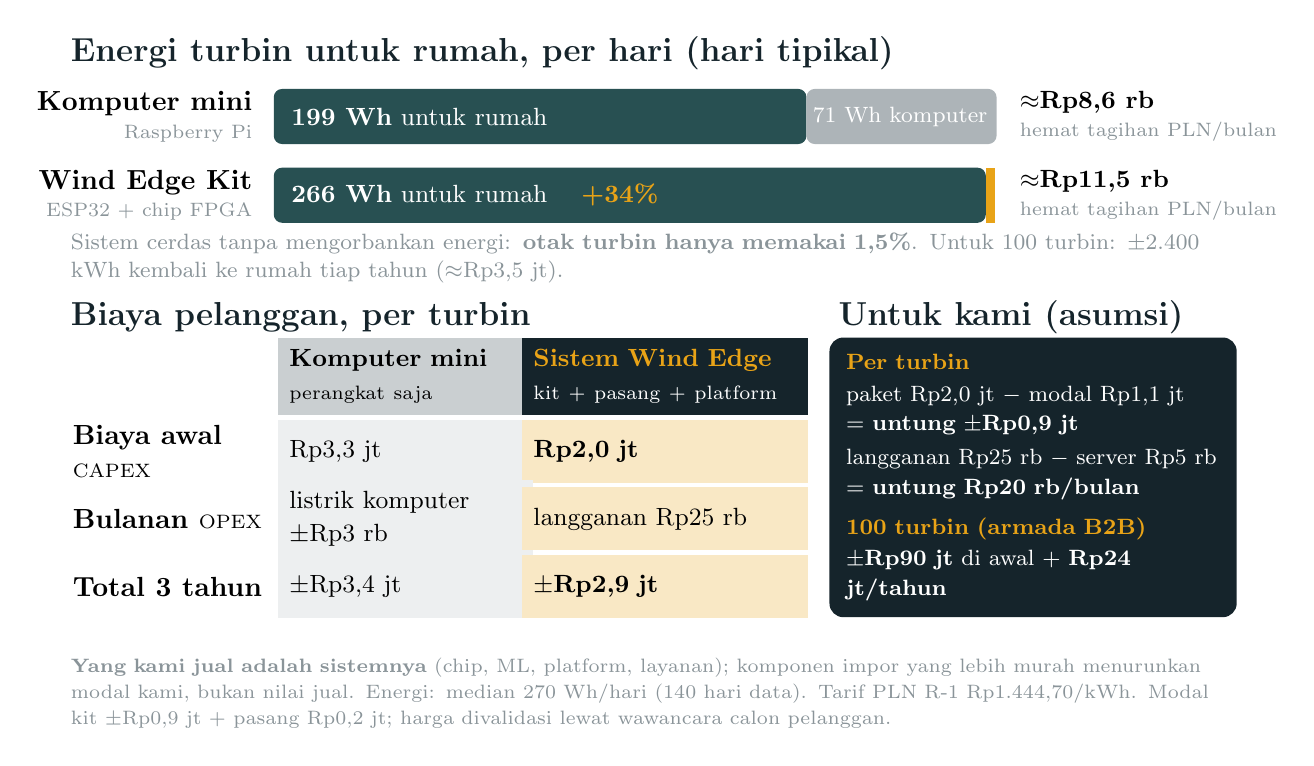
\begin{tikzpicture}[font=\fontsize{9.5}{12}\selectfont,
  sel/.style={minimum height=0.8cm, text width=#1, align=left, inner sep=4pt, anchor=west}]
  % ---------- atas: energi turbin untuk rumah
  \def\s{0.034}  % cm per Wh (270 Wh = 9,18 cm)
  \node[anchor=west, font=\judulfont\bfseries\fontsize{11.5}{13}\selectfont, text=gelap] at (0,4.55) {Energi turbin untuk rumah, per hari (hari tipikal)};
  \node[anchor=east, align=right, font=\bfseries] at (2.55,3.75) {Komputer mini\\[-2pt]{\mdseries\fontsize{7.5}{9}\selectfont\color{abu}Raspberry Pi}};
  \fill[teal, rounded corners=3pt] (2.7,3.4) rectangle ++(199*\s,0.7);
  \fill[abu!70, rounded corners=3pt] (2.7+199*\s,3.4) rectangle ++(71*\s,0.7);
  \node[text=white, anchor=west] at (2.8,3.75) {\textbf{199 Wh} untuk rumah};
  \node[text=white, font=\fontsize{8}{9}\selectfont] at (2.7+234*\s,3.75) {71 Wh komputer};
  \node[anchor=west, align=left] at (12.05,3.75) {$\approx$\textbf{Rp8,6 rb}\\[-2pt]{\fontsize{7.5}{9}\selectfont\color{abu}hemat tagihan PLN/bulan}};
  \node[anchor=east, align=right, font=\bfseries] at (2.55,2.75) {Wind Edge Kit\\[-2pt]{\mdseries\fontsize{7.5}{9}\selectfont\color{abu}ESP32 + chip FPGA}};
  \fill[teal, rounded corners=3pt] (2.7,2.4) rectangle ++(266*\s,0.7);
  \fill[amber] (2.7+266*\s,2.4) rectangle ++(0.12,0.7);
  \node[text=white, anchor=west] at (2.8,2.75) {\textbf{266 Wh} untuk rumah \quad {\color{amber}\bfseries +34\%}};
  \node[anchor=west, align=left] at (12.05,2.75) {$\approx$\textbf{Rp11,5 rb}\\[-2pt]{\fontsize{7.5}{9}\selectfont\color{abu}hemat tagihan PLN/bulan}};
  \node[anchor=west, text=abu, font=\fontsize{8}{10}\selectfont, text width=14.6cm] at (0,1.95)
    {Sistem cerdas tanpa mengorbankan energi: \textbf{otak turbin hanya memakai 1,5\%}. Untuk 100 turbin: $\pm$2.400 kWh kembali ke rumah tiap tahun ($\approx$Rp3,5 jt).};
  % ---------- bawah kiri: biaya pelanggan
  \node[anchor=west, font=\judulfont\bfseries\fontsize{11.5}{13}\selectfont, text=gelap] at (0,1.2) {Biaya pelanggan, per turbin};
  \node[sel=2.95cm, fill=abu!45, minimum height=0.95cm] at (2.75,0.45) {{\bfseries Komputer mini}\\{\fontsize{7.5}{9}\selectfont perangkat saja}};
  \node[sel=3.35cm, fill=gelap, text=white, minimum height=0.95cm] at (5.85,0.45) {{\bfseries\color{amber}Sistem Wind Edge}\\{\fontsize{7.5}{9}\selectfont kit + pasang + platform}};
  \def\baris#1#2#3#4{%
    \node[sel=2.55cm, font=\bfseries] at (0,#1) {#2};
    \node[sel=2.95cm, fill=abu!15] at (2.75,#1) {#3};
    \node[sel=3.35cm, fill=amber!25] at (5.85,#1) {#4};}
  \baris{-0.5}{Biaya awal {\mdseries\fontsize{7.5}{9}\selectfont CAPEX}}{Rp3,3 jt}{\textbf{Rp2,0 jt}}
  \baris{-1.36}{Bulanan {\mdseries\fontsize{7.5}{9}\selectfont OPEX}}{listrik komputer $\pm$Rp3 rb}{langganan Rp25 rb}
  \baris{-2.22}{Total 3 tahun}{$\pm$Rp3,4 jt}{\textbf{$\pm$Rp2,9 jt}}
  % ---------- bawah kanan: untung kami
  \node[anchor=west, font=\judulfont\bfseries\fontsize{11.5}{13}\selectfont, text=gelap] at (9.75,1.2) {Untuk kami (asumsi)};
  \node[anchor=north west, fill=gelap, text=white, rounded corners=5pt, text width=4.75cm, inner sep=6pt, font=\fontsize{8.5}{10.5}\selectfont] at (9.75,0.95) {%
    \textbf{\color{amber}Per turbin}\\[1pt]
    paket Rp2,0 jt $-$ modal Rp1,1 jt\\= \textbf{untung $\pm$Rp0,9 jt}\\[2pt]
    langganan Rp25 rb $-$ server Rp5 rb\\= \textbf{untung Rp20 rb/bulan}\\[4pt]
    \textbf{\color{amber}100 turbin (armada B2B)}\\[1pt]
    \textbf{$\pm$Rp90 jt} di awal + \textbf{Rp24 jt/tahun}};
  \node[anchor=north west, text width=14.6cm, font=\fontsize{7.5}{9.5}\selectfont, text=abu] at (0,-3.0)
    {\textbf{Yang kami jual adalah sistemnya} (chip, ML, platform, layanan); komponen impor yang lebih murah menurunkan modal kami, bukan nilai jual.
     Energi: median 270 Wh/hari (140 hari data). Tarif PLN R-1 Rp1.444,70/kWh. Modal kit $\pm$Rp0,9 jt + pasang Rp0,2 jt; harga divalidasi lewat wawancara calon pelanggan.};
\end{tikzpicture}
\end{document}
